% !TEX program = lualatex
% !TEX encoding = UTF-8 Unicode
% 
\newcommand{\titol}{Sistemas basados en el conocimiento}
\newcommand{\materia}{Inteligencia artificial}
\newcommand{\idioma}{english,spanish}
\newcommand{\pdfauthors}{Nil Mamano Grande, Héctor Ramón Jiménez, Isaac Sánchez Barrera}
%\newcommand{\autors}[1]{\begin{tabular}{#1} Nil Mamano Grande \\ Héctor Ramón Jiménez \\ Isaac Sánchez Barrera\end{tabular}}
\newcommand{\autors}[1]{\begin{tabular}{#1} Mamano -- Ramón -- Sánchez\end{tabular}}
\newcommand{\data}{\today}
% !TEX encoding = UTF-8 Unicode
% !TEX root = report.tex
% 
\documentclass[a4paper,10pt,twoside,titlepage,abstract,numbers=noenddot,automark,mnsy,intlimits,rgb,dvipsnames]{scrartcl}
%\usepackage[utf8]{inputenc}
\usepackage{csquotes}
\usepackage[\idioma, es-tabla]{babel}
\spanishdecimal{.}
\usepackage{fontspec}
\defaultfontfeatures{Scale=MatchLowercase, Ligatures=TeX}
\usepackage{pdfpages}
\usepackage{fancyvrb}
\usepackage{amssymb}
\usepackage{amsmath}
\usepackage{mathtools}
\usepackage{unicode-math}
\unimathsetup{math-style=ISO,vargreek-shape=unicode}
\usepackage{xunicode}
\usepackage{ifxetex}
\usepackage{algorithm}
\usepackage{algpseudocode}

\ifxetex
  \usepackage{xltxtra}
\fi
\usepackage{verbatim}

\usepackage[binary-units]{siunitx}
\sisetup{
  product-units=single,
  list-units=single,
  per-mode=symbol,
  list-final-separator = { y },
  list-pair-separator = { y },
  range-phrase = { a },
}

\usepackage{fullpage}
\usepackage{framed}
\usepackage{xfrac}

\defaultfontfeatures{Path=fonts/, Scale=MatchLowercase}
\setmainfont[Ligatures=TeX,
BoldFont=texgyrepagella-bold.otf,
BoldItalicFont=texgyrepagella-bolditalic.otf,
ItalicFont=texgyrepagella-italic.otf]{texgyrepagella-regular.otf} %use this font
\setsansfont[Ligatures=TeX,
BoldFont=lmsans10-bold.otf,
BoldItalicFont=lmsans10-boldoblique.otf,
ItalicFont=lmsans10-oblique.otf]{lmsans10-regular.otf}
\setmonofont[BoldFont=lmmonolt10-bold.otf,
BoldItalicFont=lmmonolt10-boldoblique.otf,
ItalicFont=lmmono10-italic.otf,
SlantedFont=lmmonoslant10-regular.otf]{lmmono10-regular.otf}
\setmathfont{texgyrepagella-math.otf}
\setmathfont[range={\mathcal,\mathbfcal},StylisticSet=1]{xits-math.otf}

\usepackage[super]{nth}
%\setmathfont[ Path=fonts/, ]{LM Math}
%\usepackage{natbib}
\usepackage[natbib=true,language=english,style=numeric,citestyle=numeric,bibstyle=numeric,hyperref=true]{biblatex}

\usepackage{url}
\usepackage{pdflscape}
\usepackage{enumitem}

\usepackage{graphicx}
\usepackage{float}
\usepackage{caption}
\usepackage{subcaption}
\usepackage{multicol}
\usepackage{booktabs}

\usepackage[hidelinks]{hyperref}
\hypersetup{
    pdfencoding=auto,
    pdffitwindow=false,      % page fit to window when opened
    pdftitle={\materia\ :: \titol},    % title
    pdfauthor={\pdfauthors},     % author
    pdfsubject={},   % subject of the document
    pdfcreator={XeLaTeX + Hyperref package},
    colorlinks=false
}

\usepackage{setspace}

\usepackage[nouppercase]{scrpage2}

\setlength{\headheight}{15pt}
\renewcommand{\headfont}{\upshape}
\defpagestyle{curr}
  {    %% superior
    (\textwidth,0pt) %líneas
    {    %%par
      {\autors{l}}
      {\hfill}
      {\leftmark}
    }
    {	%%impar
      {\rightmark}
      {\hfill}
      {\autors{r}}
    }
    {	%% una sola cara
      {\thepart}
      {\hfill}
      {\autors{r}}
    }
    (\textwidth,0.5pt) %líneas
  }
  {		%% inferior
    (\textwidth,0.5pt) %líneas
    {	%%par
      {\thepage}
      {\hfill}
      {\materia}
    }
    {	%%impar
      {\titol}
      {\hfill}
      {\thepage}
    }
    {	%% una sola cara
      {\materia: \titol}
      {\hfill}
      {\thepage}
    }
    (\textwidth,0pt) %líneas
  }

\pagestyle{curr}

\headsep = 15pt
%\addtolength{\footskip}{-16pt}
%\addtolength{\textheight}{+16pt}
\addtolength{\topmargin}{-15pt}
\addtolength{\hoffset}{12mm}
\addtolength{\textwidth}{-11mm}
\usepackage{wrapfig}

\usepackage{amsthm}
%~ \theoremprework {\textcolor{white} {\rule{0.2in}{0.11in}} \hrule\rule{0.2in}{0.11in}}
%~ \theorempostwork {\hrule %\textcolor{white} {\rule{0.2in}{0.11in}}
%~ }

\makeatletter
\newcommand{\strong}[1]{\@strong{#1}}
\newcommand{\@@strong}[1]{\textbf{\let\@strong\@@@strong#1}}
\newcommand{\@@@strong}[1]{\textnormal{\let\@strong\@@strong#1}}
\let\@strong\@@strong
\makeatother

%~ \theoremindent0.5cm
%~ \theoremstyle{break}
%~ \theorembodyfont{}
%~ \newtheorem*{defi}{}

\theoremstyle{plain}% default
\newtheorem{thm}{Teorema}[section]
\newtheorem{lem}[thm]{Lemma}
\newtheorem{prop}{Proposition}
\newtheorem{cor}{Corollary}

\theoremstyle{definition}
\newtheorem{defn}{Definition}[section]
\newtheorem{conj}{Conjecture}[section]
\newtheorem{exmp}{Example}[section]

\theoremstyle{remark}
\newtheorem*{obs}{Observation}
\newtheorem*{note}{Remark}
\newtheorem{case}{Case}
\newtheorem*{notation}{Notation}

\addtolength{\voffset}{-15pt}
\addtolength{\headsep}{10pt}
\addtolength{\textheight}{35pt}
\addtolength{\footskip}{-20pt}
\addtolength{\textwidth}{15pt}
\addtolength{\marginparwidth}{-20pt}
\addtolength{\oddsidemargin}{-20pt}
\addtolength{\evensidemargin}{-20pt}

\usepackage{listings}

\definecolor{FonsCodi}{cmyk}{0,0,0,0.04}
\definecolor{Comentaris}{cmyk}{0,0,0,0.6}
\definecolor{mygreen}{rgb}{0,0.6,0}
\definecolor{mygray}{rgb}{0.6,0.6,0.6}
\definecolor{mymauve}{rgb}{0.58,0,0.82}
\definecolor{darkgreen}{rgb}{0.2,0.5,0.2}
\definecolor{orange}{rgb}{1,0.5,0}

\lstset{ %
language=Java,                % choose the language of the code
basicstyle=\ttfamily\small,
numbers=none,                   % where to put the line-numbers
numberstyle=\footnotesize,      % the size of the fonts that are used for the line-numbers
stepnumber=1,                   % the step between two line-numbers. If it's 1 each line will be numbered
numbersep=5pt,                  % how far the line-numbers are from the code
backgroundcolor=\color{FonsCodi},  % choose the background color. You must add \usepackage{color}
rulesepcolor=\color{FonsCodi},
lineskip=-2.5pt,
showspaces=false,               % show spaces adding particular underscores
showstringspaces=false,         % underline spaces within strings
showtabs=false,                 % show tabs within strings adding particular underscores
frame=single,                    % adds a frame around the code
tabsize=8,	                % sets default tabsize to 2 spaces
commentstyle=\itshape\color{Comentaris},
captionpos=t,                   % sets the caption-position to top
breaklines=true,                % sets automatic line breaking
breakatwhitespace=false,        % sets if automatic breaks should only happen at whitespace
escapeinside={\%*}{*)},          % if you want to add a comment within your code
keywordstyle=\bfseries\color{blue},
commentstyle=\itshape\color{darkgreen},
stringstyle=\color{orange},
}

\renewcommand{\lstlistlistingname}{Índice de códigos fuente}
\renewcommand{\lstlistingname}{Código fuente}

\setstretch{1.0}
\DefineBibliographyStrings{spanish}{%
  references = {Referencias},
}

\title{\materia\\
\Large{\titol}}
\subtitle{Facultat d'Informàtica de Barcelona\\ % Pongo la I mayúscula porque la FIB lo hace
Universitat Politècnica de Catalunya}
\author{
  Nil Mamano Grande \\
  Héctor Ramón Jiménez \\
  Isaac Sánchez Barrera}
\date{
  \today \\
  cuatrimestre de otoño \\
  curso 2013--2014}

\everymath{\displaystyle}

\newcommand{\CC}{\mathbb{C}}
\newcommand{\RR}{\mathbb{R}}
\newcommand{\NN}{\mathbb{N}}
\newcommand{\bigO}[1]{\ensuremath{\operatorname{O}\left(#1\right)}}% big-O notation/symbol
\newcommand{\bigOmega}[1]{\ensuremath{\operatorname{\Omega}\left(#1\right)}}% big-O notation/symbol
\newcommand{\bigTheta}[1]{\ensuremath{\operatorname{\Theta}\left(#1\right)}}% big-O notation/symbol
\newcommand{\slot}[1]{\textsl{\texttt{#1}}}
\newcommand{\clase}[1]{\texttt{#1}}
\newcommand{\regla}[1]{\textsl{\texsf{#1}}}

\newenvironment{slotlist}{%
   \renewcommand\descriptionlabel[1]{\hspace{\labelsep}\slot{##1}}
   \begin{description}%
}{%
   \end{description}%
}

\bibliography{references}
\begin{document}

\maketitle
\tableofcontents
\listoftables
\listoffigures
\vfill
\cleardoublepage

\part{Presentación y análisis del problema}
% !TEX encoding = UTF-8 Unicode
% !TEX root = ../report.tex
% 

\begin{wrapfigure}{O}{0.3\textwidth}
  \vspace{-20pt}
  \begin{center}
    
\includegraphics[width=0.28\textwidth]{figures/ricorico}
  \end{center}
  \vspace{-20pt}
\end{wrapfigure}

\section{Introducción}
\subsection{Descripción del problema}
La empresa de catering \emph{Rico Rico} quiere mejorar su eficiencia a la hora
de proponer menús para las celebraciones de sus clientes. Con ese fin, ha
encargado la implementación de un sistema experto basado en el conocimiento que
tienen tras su larga experiencia en el sector. Gracias al sistema, solamente es
necesario que el cliente indique sus preferencias y restricciones concretas
para obtener las recomendaciones más acordes con sus necesidades.



% !TEX encoding = UTF-8 Unicode
% !TEX root = ../report.tex
% 

\section{Conceptualización del problema}
\subsection{Conceptos principales del dominio}

Después de haber hecho un trabajo iterativo, los conceptos que se modelan en el
dominio de conocimiento son
\begin{enumerate}
  \item Cosas elaboradas, como platos y vino (tienen su nombre y precio).
  \item Dentro de los platos, si son pesados o ligeros y su dificultad de
    preparación.
  \item Los ingredientes que forman parte de los platos y su disponibilidad
    durante las cuatro estaciones del año.
  \item Grandes grupos de comensales, que modelan el tipo de ingredientes que
    no pueden comer.
  \item Los tipos de platos, que contienen información sobre los vinos que
    pueden ir mejor con ellos.
  \item Los eventos a celebrar, que tienen los platos que son propios (o
    recomendables) y la importancia de éstos últimos a la hora de elaborar el
    los menús para el cliente.
  \item Las regiones de procedencia de los platos.
  \item El estilo de los platos. Están los genéricos, que no llegarían a ser
    tradicionales porque son simples platos, los tradicionales (podrían
    considerarse, en parte, folclóricos), y platos modernos. Además, también se
    hace distinción de los platos para sibaritas, que son para los paladares
    más finos, pero que pueden pertenecer a cualquiera de las categorías
    anteriores.
\end{enumerate}

Como hemos indicado anteriormente, los comensales que no beben vino acostumbran
a preferir una bebida concreta de forma individualizada. Por esta razón, hemos
pensado que no es algo a modelar en nuestro dominio de conocimiento.

Por otro lado, en el dominio de solución disponemos de
\begin{enumerate}
  \item Recomendaciones concretas de platos, con los motivos para su
    recomendación y una valoración.
  \item Posibles menús abstractos, que contienen el orden de platos y los
    colores de los vinos más aptos para éstos.
  \item Los menús finales con los platos y vinos concretos, además de las
    razones y valoración de su recomendación.
\end{enumerate}

\vfill
\clearpage
\part{Implementación del sistema experto}
% !TEX encoding = UTF-8 Unicode
% !TEX root = ../report.tex
% 

\section{Construcción de la ontología}

\begin{figure}[h!]
  \makebox[\textwidth][c]{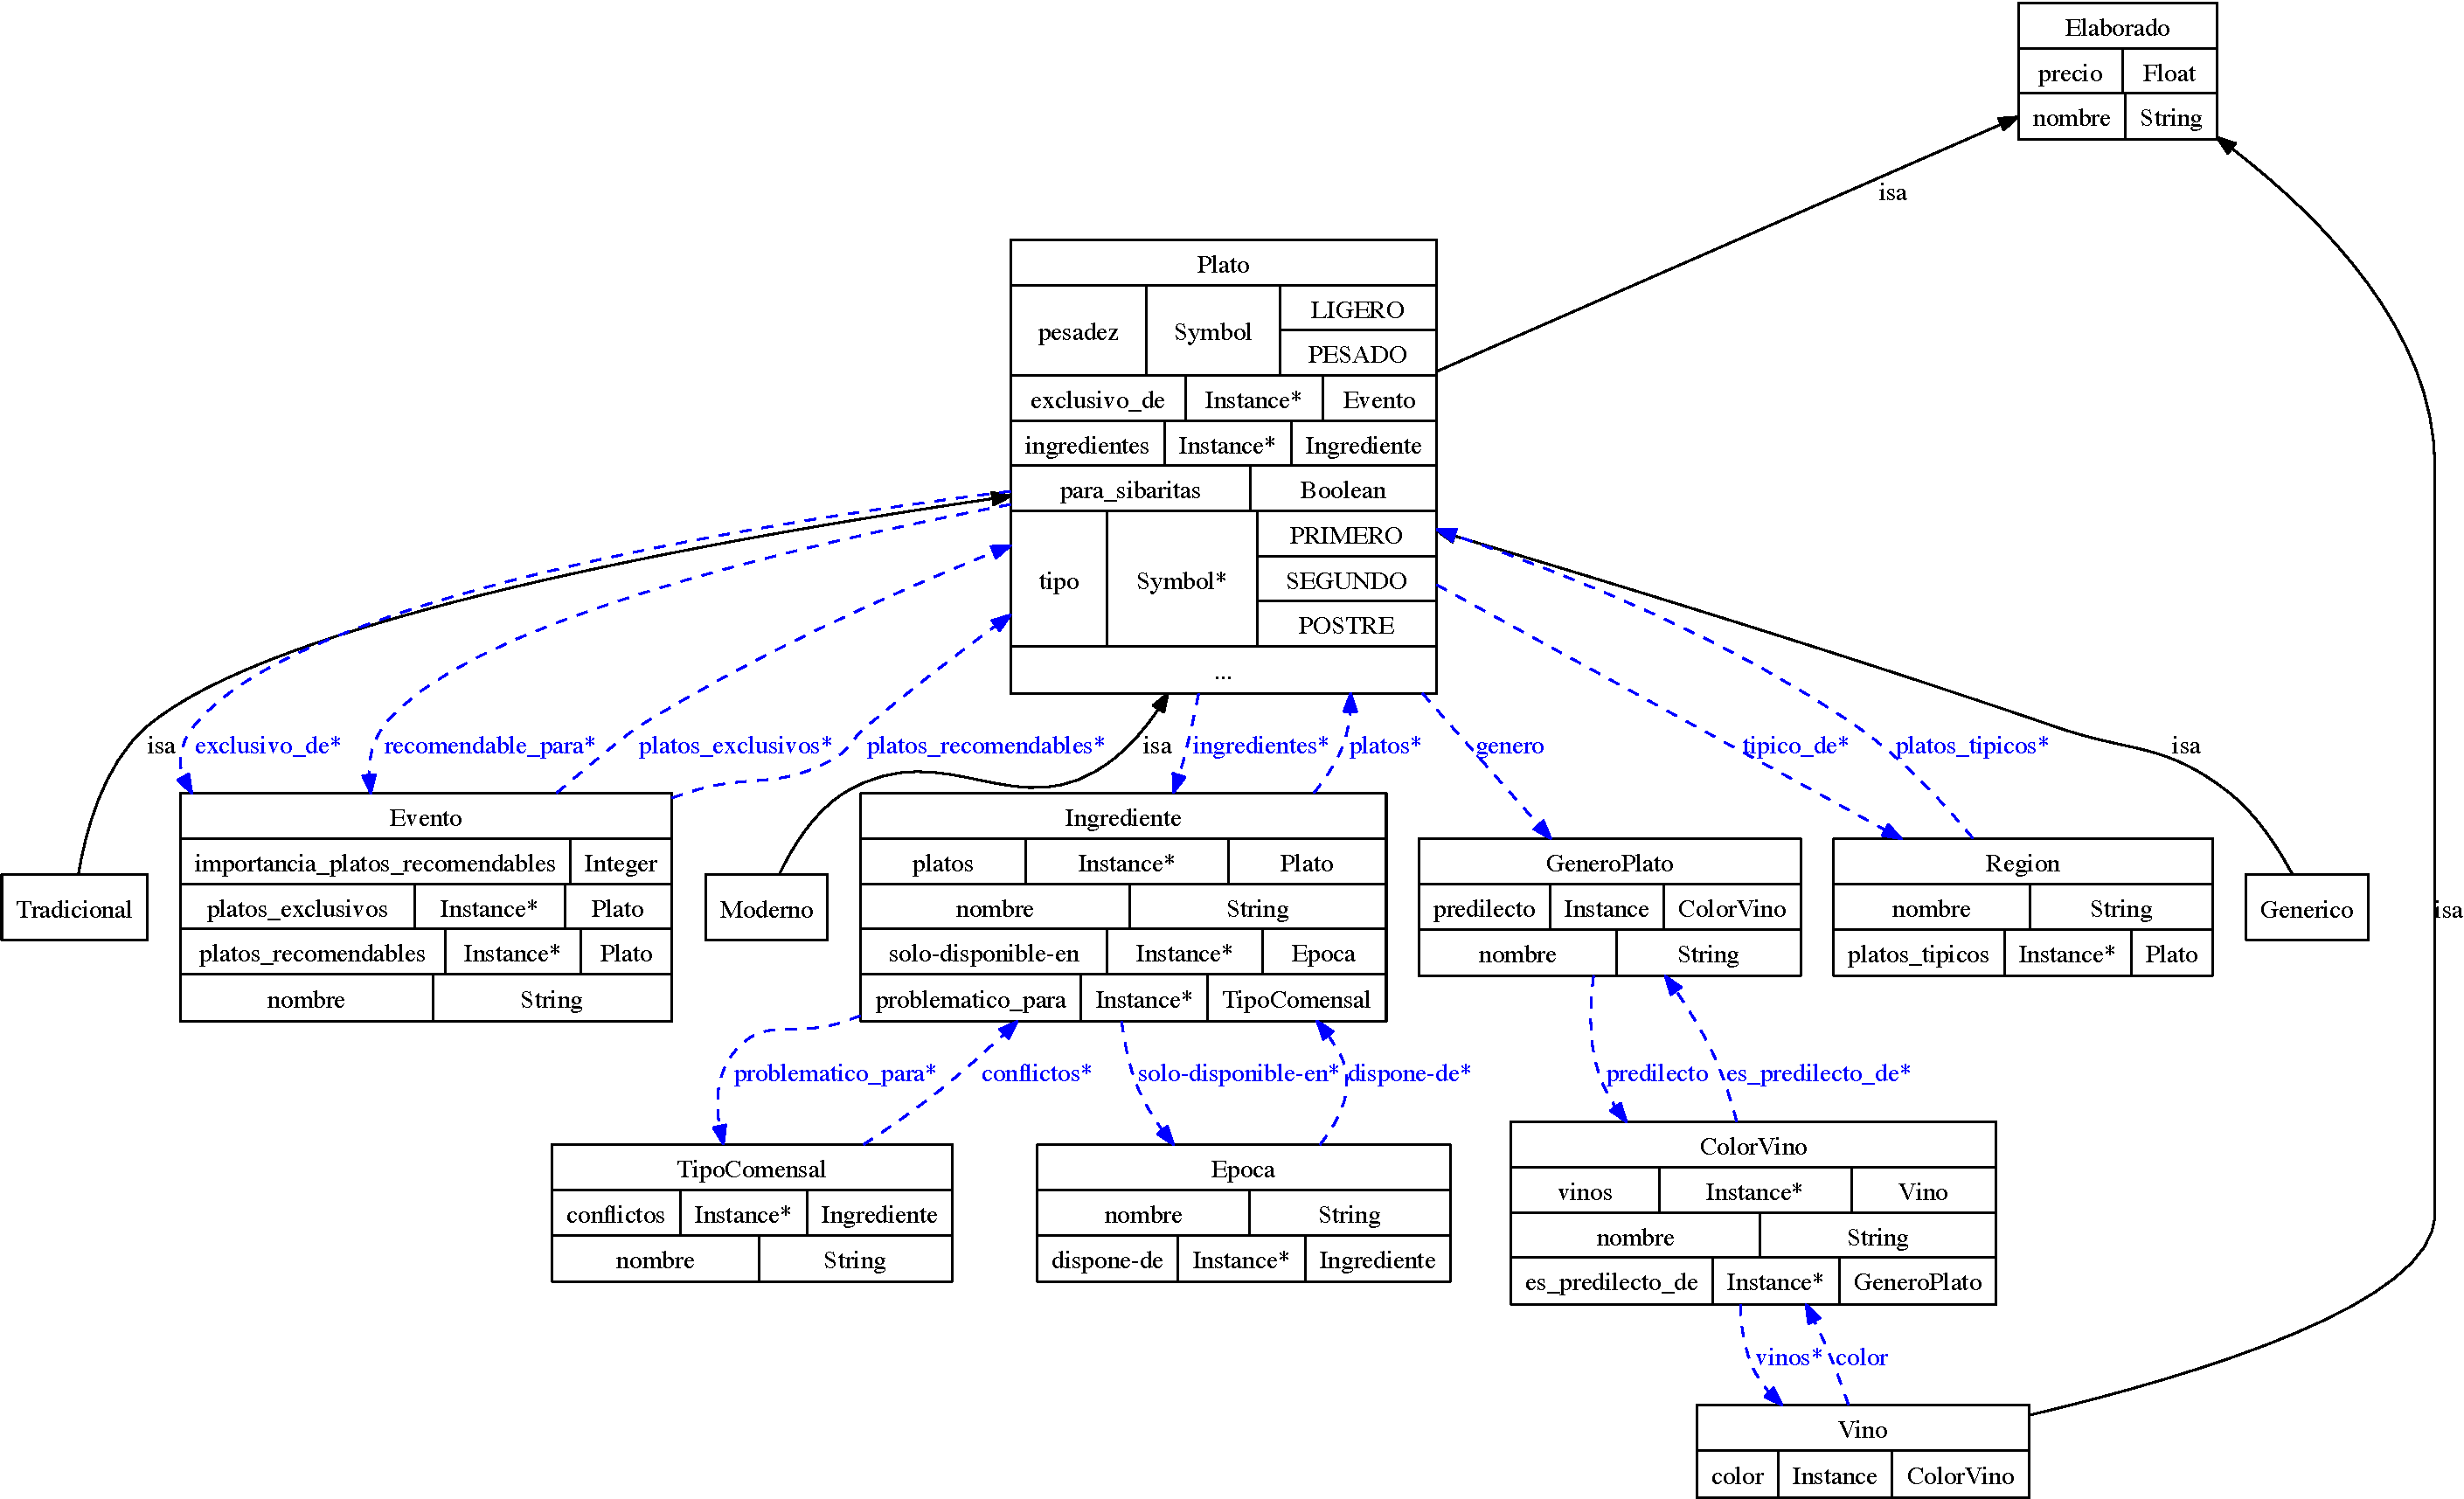
\includegraphics[width=1.2\textwidth]{%
      figures/ontologia}}
  \caption{La ontología final}
\end{figure}

La construcción de la ontología (y de todo el sistema en general) se ha
realizado de manera iterativa, aunque inicialmente no había sido así.

En un principio habíamos construido sistema de clases completo pero incluso más
complejo de lo que ha sido finalmente, sin necesidad. Afortunadamente, esa
versión se perdió y empezamos con una más simple que solamente contenía las
clases elaborado, plato, bebida (que ahora es solamente vino) e ingrediente.

Luego añadimos la clase de tipos de comensal, para poder tener en cuenta
alergias y demás problemas alimenticios. También se añadió la clase época para
poder indicar la disponibilidad de ingredientes.

Inicialmente, los eventos iban a ser unos valores prefijados hasta que vimos
que podríamos sacarle más provecho a todo si eran instancias dentro de la
ontología. Así que creamos la clase evento y asociamos algunos platos como
preferidos en el evento. Para evitar que determinados platos propios de un
evento se recomendaran en otros donde no tuviera sentido (un claro ejemplo son
los pasteles de boda), casi al final hicimos la diferencia entre platos propios
y platos que son recomendables para los eventos.

Ya, más entrados en el proceso de implementación del sistema experto, añadimos
la clase región para poder modelar el origen geográfico/cultural de los
platos. Finalmente, cuando empezamos a tratar con los vinos, y tras considerar
que la bebida en general no tiene sentido para el problema que se nos pide
resolver, eliminamos la clase bebida, dejando solamente una clase para
vinos. Además, creamos la clase que modela el color del vino, que se asoció a
la nueva clase de géneros de plato (sopa, pescado, estofado, aperitivo, etc.)
para poder hacer la recomendación de vinos de manera más sencilla.

Fuera de aquí, también están las ontologías de solución del problema, que
solamente contienen las clases menú y menú abstracto. Más adelante detallaremos
su funcionamiento.

\subsection{Detalle de las clases de la ontología del problema}
\subsubsection{Clase \texttt{Elaborado}}
Esta clase está construida para agrupar las características propias de los
productos que se venden con el menú: el \slot{nombre} y el
\slot{precio}. La idea es que cualquier cosa que esté en el menú debe ser un
producto elaborado.

En determinado momento tuvimos que hacer esta clase concreta para poder hacer
\emph{pattern matching} con CLIPS. Por suerte, los cambios que fuimos haciendo
en la implementación del problema provocaron que esta clase pudiera volver a
ser abstracta. Mientras la clase fue concreta, la clase \verb+Plato+ también
tuvo que serlo porque CLIPS no permite subclases abstractas de clases
concretas.

\subsubsection{Clase \texttt{Plato} y sus subclases}
La clase es abstracta y está dividida en las subclases \verb+Generico+,
\verb+Moderno+ y \verb+Tradicional+. Hemos decidido hacer esta clasificación
porque no es habitual que un plato sea moderno y tradicional a la vez, y
también existen platos que no se considerarían tradicionales pero que son
platos que se consumen habitualmente (de ahí el término genérico).

Además del nombre y el precio derivados de \verb+Elaborado+, la clase
\verb+Plato+ proporciona nuevos campos:
\begin{slotlist}
\item[ingredientes] Es un campo múltiple de instancias de la clase
  \verb+Ingrediente+. Es necesario que haya como mínimo un ingrediente.
\item[genero] Es un campo simple que apunta a una instancia de
  \verb+GeneroPlato+. Sirve para clasificar los platos en sus géneros.
\item[tipo] Un campo múltiple que indica si el plato es \emph{primero},
  \emph{segundo} o \emph{postre}. Es necesario que sea algún tipo de plato.
\item[para\_sibaritas] Un campo cierto/falso. Los platos para sibaritas no
  queremos que se recomienden a alguien que no lo es, pues es habitual que no
  lo quieran. Por otro lado, se les da prioridad si el cliente sí lo es.
\item[temperatura] Indica si el plato es frío o caliente.
\item[pesadez] Indica si un plato es ligero o pesado. En general, no es bueno
  que un cliente coma dos platos ligeros o dos platos pesados.
\item[tipico\_de] Es un campo múltiple que contiene las instancias de
  \verb+Region+ de donde es típico el plato, si es el caso.
\item[recomendable\_para] Un campo múltiple que contiene, si es el caso, en qué
  eventos pueden preferir el plato, para que se priorice.
\item[exclusivo\_de] A diferencia del anterior, si está definido indica en qué
  eventos puede ofrecerse el plato de forma exclusiva (por ejemplo, un pastel
  de boda solamente puede ofrecerse en una boda). También lo prioriza.
\item[dificultad] Indica, mediante un valor de 0 a 100, la dificultad de
  elaboración del plato (un valor mayor indica una dificultad mayor). Cuantos
  más comensales hay en la celebración, más importante es que el plato sea más
  sencillo de elaborar.
\end{slotlist}

Las subclases de \verb+Plato+ no contienen ningún slot propio. Simplemente es
para poder separar correctamente y poder hacer uso del \emph{pattern matching}
en CLIPS.

\subsubsection{Clase \texttt{GeneroPlato}}
Mediante esta clase se modelan los distintos géneros de plato en función de
cómo son. Es decir, sopas, platos de pescado, estofados, etc. Se utiliza para
poder agrupar platos similares que precisan vinos de colores similares. Por
tanto, además del \slot{nombre} del género, el único campo que tienen es
\slot{predilecto}, que apunta al color de vino más acorde con los platos de ese
género.

No tienen el campo inverso hacia \verb+Plato+ con los platos del género porque
no lo usamos durante el problema.

\subsubsection{Clase \texttt{Vino}}
Esta clase representa a los vinos. Además de los campos de \verb+Elaborado+,
contiene un campo \slot{color} que apunta a la instancia de \verb+ColorVino+
con el color del vino.

\subsubsection{Clase \texttt{ColorVino}}
Como ya hemos comentado con anterioridad, esta clase representa los colores que
puede tomar un vino. Los campos que tiene, además del \slot{nombre} del color, son dos:
\begin{slotlist}
\item[es\_predilecto\_de] Es el campo múltiple que contiene la lista de géneros
  de plato que prefieren ese color de vino. Por tanto, es el inverso del campo
  \verb+ColorVino+:\slot{predilecto}.
\item[vinos] Este campo múltiple guarda la lista de vinos del color. Es el campo inverso a \verb+Vino+:\slot{color}.
\end{slotlist}

% !TEX encoding = UTF-8 Unicode
% !TEX root = ../report.tex
% 

\section{Formalización e implementación del sistema experto mediante \texttt{CLIPS}}

% !TEX encoding = UTF-8 Unicode
% !TEX root = ../../report.tex
% 

\subsection{Módulo de abstracción de datos}
El primer módulo
% !TEX encoding = UTF-8 Unicode
% !TEX root = ../../report.tex
% 

\subsection{Módulo de platos}
Una vez se han obtenido las preferencias del cliente y el contexto del evento que se quiere realizar, se activa el
\strong{módulo de platos}.
El objetivo del \strong{módulo de platos} es seleccionar los mejores platos disponibles para celebrar el evento que el cliente ha 
descrito en el módulo de abstracción teniendo en cuenta todas sus preferencias. Este módulo está dividido en tres fases o submódulos: 
\strong{filtración}, \strong{puntuación} y \strong{selección}.

\subsubsection{Fase de filtración}
En esta primera fase se crea una \texttt{Recomendacion} por cada plato presente en la ontología. Una \texttt{Recomendacion} no es más
que un contenedor del plato en sí, más una puntuación y sus justificaciones.
A continuación, se descartan todas aquellas recomendaciones cuyos platos son incompatibles con los datos obtenidos del cliente. Más
exactamente, se eliminan las recomendaciones cuyos platos:

\begin{enumerate}
\item Contienen ingredientes prohibidos (ver apartado \ref{abstraccion-datos}).
\item Son exclusivos de un tipo de evento diferente al que se va a celebrar.
\item Son demasiado caros para las limitaciones de precio establecidas.
\item Son para los paladares más exigentes y el cliente no es sibarita.
\end{enumerate}

\subsubsection{Fase de puntuación}
Esta fase consiste en puntuar todas las recomendaciones en función de las preferencias del cliente. Cuando una recomendación
es puntuada, al mismo tiempo se le añade una justificación. De esta manera es posible ofrecer al cliente una explicación detallada
de las recomendaciones que ha recibido.

Sea $p$ un plato de una recomendación, se puntúa (por orden de prioridad):

\begin{description}
\item[Exclusivo del evento] Positivamente si $p$ es exclusivo del tipo de evento a celebrar.
\item[Recomendado para el evento] Positivamente si $p$ es recomendado para el tipo de evento a celebrar.
\item[Tipo de cocina] Positivamente si $p$ es de un tipo de cocina preferido por el cliente y negativamente si no lo es.
\item[Zonas geográficas] Positivamente si $p$ es típico de alguna de las zonas geográficas preferidas por el cliente.
\item[Sibarita] Positivamente si $p$ es para paladares exigentes y el cliente es sibarita.
\item[Temperatura] Si el cliente tiene preferencia de temperatura, positivamente si $p$ se sirve a la temperatura preferida por el cliente
y negativamente en caso contrario.
\item[Dificultad] Negativamente si $p$ supera la dificultad máxima establecida para el número de comensales del evento.
\item[Plato caliente en verano] Negativamente si $p$ se sirve caliente y el evento se celebrará en la estación de verano.
\item[Plato caliente en invierno] Positivamente si $p$ se sirve caliente y el evento se celebrará en la estación de invierno.
\end{description}

Cada aspecto del plato puntuado tiene un peso asignado que permite modificar la prioridad de unas características frente 
otras\footnote{De hecho, los pesos se encuentran centralizados en un \texttt{template} \texttt{Pesos} dentro del propio módulo de
puntuación.}. Hemos decidido darle prioridad a los platos \strong{exclusivos del evento} para asegurarnos de que platos como, por 
ejemplo, un pastel de boda siempre estén presentes en los menús recomendados para dichos eventos. Luego, hemos considerado más
importante que un plato sea del tipo de cocina preferido por el cliente antes que de una zona geográfica preferida o que se sirva a la
temperatura preferida\footnote{Una posible mejora del sistema sería preguntarle al cliente la prioridad que quiere dar a cada una de
sus preferencias y así obtener menús todavía más personalizados.}.

\subsubsection{Fase de selección}
Una vez los platos ya han sido puntuados se pasa a la \strong{fase de selección}. En esta fase se seleccionan los
\strong{30 mejores primeros}, los \strong{30 mejores segundos} y los \strong{15 mejores postres}. Si no hiciéramos esto el
sistema no sería escalable, ya que el número de menús tiene crecimiento cúbico respecto al número de primeros, segundos y postres.
La cantidad de platos de cada tipo seleccionados\footnote{Se seleccionan menos postres porque es más normal que haya repetición de platos entre los primeros y los segundos.} permite para poder generar menús con la suficiente diversidad sin que se dispare
el número de combinaciones aunque se añadan más platos a la ontología.

% !TEX encoding = UTF-8 Unicode
% !TEX root = ../../report.tex
% 

\subsection{Módulo de menús}
Una vez se han seleccionado los hasta 30 primeros platos, 30 segundos y 15
postres, llega el momento de empezar a combinarlos para crear los menús.

El módulo de menús está dividido en tres fases (tres módulos de \texttt{CLIPS})
y se encarga de generar, puntuar y seleccionar los menús abstractos que pasarán
al módulo de vinos. A continuación podremos ver los detalles de su
funcionamiento.

Originalmente hacíamos las combinaciones con los vinos directamente, sin usar
la clase \clase{MenuAbstracto} con \clase{ColorVino}. El problema es que se
producía una explosión combinatoria muy grande sin necesidad, ya que
originalmente el sistema no usaba nada más que el color del vino para valorar
la combinación del vino con los platos.

\subsubsection{Fase de filtración}
Antes que nada, una vez se tienen las instancias de \clase{Recomendacion} para
primeros, segundos y postres, se realizan todas las combinaciones posibles
junto con instancias de \clase{ColorVino}, si el cliente así lo ha
solicitado. Todas estas combinaciones se guardan como instancias de
\clase{MenuAbstracto}.

Hay una serie de menús que querríamos evitar, porque no interesa que estén en
el sistema. Si entre los platos de \strong{primero}, \strong{segundo} o
\strong{postre} que hay en la combinación que se está estudiando hay alguno
repetido, se desecha la combinación. Así que en la única regla importante la
fase, \regla{generar-menus}, se tiene en cuenta y ya directamente no se crean
dichas instancias de \clase{MenuAbstracto}.

Por otro lado, hay que tener en cuenta si el cliente ha pedido recomendaciones
de vino y, además, cuántas (una para el menú o una por plato). Por cada vino
solicitado, y por cada combinación de colores preferidos por el cliente, se
crea un menú abstracto.

Con esto, llegamos a la conclusión de que, en función de la cantidad de vinos
solicitados y los colores favoritos, podemos generar la siguiente cantidad de
menús abstractos (considerando $c$ la cantidad de colores de vino que acepta el cliente, siendo el mínimo 1 y el máximo 3):
\begin{itemize}
\item Si no se ha pedido vino, un total de como máximo $30 \times 30 \times 15
  = 13500$ menús abstractos;
\item si se ha pedido un vino, $13500 \times c$ menús abstractos;
\item y si se ha solicitado un vino por plato, $13500 \times c^2$.
\end{itemize}

Por tanto, como máximo habrá $13500 \times 9 = 121500$ menús abstractos al
acabar la fase. En la práctica habrá menos, ya que muchos platos de la
ontología pueden ser tanto primeros como segundos.

\subsubsection{Fase de puntuación}
Cuando ya se han generado todos los menús posibles, llega el momento de
puntuarlos para decidir cuáles son mejores. Para ello, definimos un
\verb+template+ (hecho no ordenado) \clase{Pesos} con la importancia del
resultado de cada regla.

Lo esencial es crear la puntuación básica del menú, y eso lo hace la regla
\regla{puntuar-menu-platos} sumando los puntos de las recomendaciones que están
como primero, segundo y postre de la instancia de \clase{MenuAbstracto} que se
está tratando.

Luego, cuando ya hay una primera cualificación del menú, \strong{se valora
  negativamente} que el primer y el segundo plato sean \strong{ambos ligeros} o
\strong{pesados}. En el primer caso, los comensales pueden no saciarse, y en el
segundo caso es por razones de salud y ahorro. 

También es necesario \strong{valorar la combinación del vino con los
  platos}. Si solamente hay una posibilidad de vino, se valora positivamente
que ambos platos encajen bien con su color. Si el cliente ha solicitado dos, se
valora que cada color de la combinación que hay en el \clase{MenuAbstracto} en
cuestión sea correcto para su plato respectivo. Es decir, el primer color con
el primer plato y el segundo color con el segundo plato.

Durante las pruebas del sistema nos dimos cuenta de que \strong{en ocasiones se
  ofrecían platos con precios muy dispares}. Si se propone un menú con un plato
que es considerablemente más caro que el otro (sin tener en cuenta el postre),
el cliente puede pensar que el menú no se ha elaborado con el suficiente
cuidado y no verlo correcto. Por ese motivo, cuando la diferencia de precio en
valor absoluto y con redondeo al entero más próximo por defecto es mayor a 1,
se resta una cantidad (5 en nuestro caso) por unidad de diferencia.

No pasa nada porque todas las combinaciones reciban alguna puntuación
negativa. En el caso de la diferencia de precios, solamente se utiliza para
afinar las recomendaciones de menús. Si una es mucho mejor que el resto, no se
verá afectada en exceso.

\subsubsection{Fase de selección}
Cuando los menús abstractos están ya todos puntuados, hay que seleccionar las
combinaciones que pasarán al módulo de vinos. No es útil utilizarlas todas
porque, para empezar, la cantidad puede ser excesiva al combinarlas con las
instancias de \clase{Vino} de la ontología y, por otro lado, muchas de las
combinaciones en los menús abstractos pueden ser realmente malas en comparación
con las que tienen mayor puntuación.

El sistema escoge los 200 mejores menús abstractos. Es un valor que se puede
cambiar, pero que ha dado unos buenos resultados de tiempo de
generación.

% !TEX encoding = UTF-8 Unicode
% !TEX root = ../../report.tex
% 

\subsection{Módulo de vinos}
Las instancias de \clase{MenuAbstracto} ya podrían servir para presentar las
propuestas de menú al usuario. Sin embargo, falta incluir los vinos concretos
si es el caso. Este módulo se encarga de eso, justamente, además de escoger los
hasta tres menús (uno barato, uno con coste medio, y uno más caro) que se
presentarán al usuario como mejores.

Para ello, se utilizan la clase \clase{Menu} y el \verb+deftemplate+
\clase{SeleccionMenus} como veremos a continuación.

\subsubsection{Fase de filtración}
Esta fase se encarga de recoger los menús abstractos que han pasado la fase de
selección del módulo de menús y combinarlos con los vinos según los colores que
haya establecidos. Además de eso, calcula el precio que tendría el menú con los
dos platos, el postre y, si es el caso, los vinos. Para el caso del vino, el
precio individual se calcula dividiendo entre 4 el precio de la botella.

La cantidad de menús que se generarán en esta fase puede ser:
\begin{itemize}
\item Si no se ha solicitado ningún vino, hasta $200$ (los mismos que menús
  abstractos);
\item si se ha solicitado un vino para el menú, como máximo $200 \times v$, con
  $v$ la cantidad de vinos que hay del color aceptado por cada menú abstracto;
\item si se ha solicitado un vino por plato, como máximo $200 \times v_1 \times
  v_2$, con los $v_i$ la cantidad de vinos de los colores por cada menú
  abstracto para el primer y segundo plato, respectivamente.
\end{itemize}

Del color que más hay es el tinto, con $12$ de las $34$ instancias. En el peor
caso, el cliente habrá solicitado un vino por plato y los 200 menús tendrán el
color tinto para ambos vinos. Como el segundo vino y el primero no pueden ser
iguales, porque el cliente ha solicitado dos vinos distintos, nos encontramos
con una cota superior de $200 \times 12 \times 11 = 26400$ menús al salir de la
fase.

\subsubsection{Fase de puntuación}
En esta fase se puntúa la combinación de los vinos con los platos. Hay que
matizar que solamente es en precio, ya que la puntuación de la corrección del
color se había hecho durante la fase de puntuación del módulo de menús.

La consideración que hemos tomado es que \strong{el vino no puede ser ni
  demasiado caro ni demasiado barato} en comparación con los platos. De forma
similar a cuando los platos tienen precios muy dispares, si el cliente obtiene
una recomendación de un plato de bajo precio con un vino muy caro, o al revés,
puede pensar que algo raro pasa con el sistema.

Consideramos que un vino es caro cuando el precio de un vaso es más caro que el
precio del plato con el que se tomará. Dicho de otro modo, si cuatro platos
cuestan menos que la botella. En ese caso, se da una puntuación negativa de 100
por cada plato del menú con los que se tomará el vino (el primero, el segundo,
o los dos según corresponda) y este último sea \emph{demasiado caro}.

De forma similar, consideramos que un vino es barato cuando (casi) tres
botellas cuestan menos que un plato con el que se tomará. En este caso, se
restan 50 puntos por cada plato con los que se tomará el vino y el último sea
\emph{demasiado barato}.

\subsubsection{Fase de selección}
Cuando ya están todos los posibles menús punutados, hay que seleccionar los
hasta tres que se presentarán al usuario (uno más barato, uno de precio
intermedio y uno más caro). Para ello, inicialmente se calculan los intervalos
de precio para los que un menú se considera barato, medio o caro.

Si el cliente no ha decidido indicar sus propios límites mínimo y máximo de
precio, se toman $0\,€$ como el mínimo y $45\,€$ como el máximo. El cálculo se
realiza dividiendo el intervalo en tres intervalos iguales. Estos cálculos se
hacen en las reglas \regla{actualizar-franja-min},
\regla{actualizar-franja-max} y \regla{actualizar-franjas-intermedias} y se
almacena su resultado en el hecho no ordenado \clase{FranjasPrecio}.

Ya en el momento de seleccionar el menú, lo que hacemos es escoger \strong{el
  menú con mejor puntuación} para \strong{cada intervalo de precios}. Si dos
menús tienen la misma puntuación y caen en el mismo rango de precios,
simplemente se toma una decisión al azar.

Cuando ha acabado esta fase, solamente hace falta presentar los resultados al
usuario.


\end{document}
